\subsection{802.11 Protocol}
Characteristics:
\begin{itemize}
    \item it is a standard ratified in 1999
    \item aim is to have a common way to allow communication between nodes
    \item it is used in WLAN indoors with various version (n/ac/\dots)\\
    $\rightarrow$ frequency used are unlicensed $\rightarrow$ 2.4/5 GHz, 900 MHz
    \item WLAN configuration with access point or ad-hoc network
    \item it defines both MAC and physical layer (radio frequency, header, size, ack, \dots)
    \item definition of some terms:
    \begin{itemize}
        \item[$\rightarrow$] DIFS (Distributed Inter Frame Space): time waiting for channel to be free\\
        $\rightarrow$ if channel is occupied $\Rightarrow$ timer restarts from the beginning\\
        (low priority $\rightarrow$ for asynchronous data service)
        \item[$\rightarrow$] SIFS (Short Inter Frame Space): time useful to process some procedures like:
        \begin{itemize}
            \item CTS (Clear To Send)
            \item Datas
            \item ACK (Acknowledgement)
        \end{itemize}
        $\Rightarrow$ high priority
        \item[$\rightarrow$] CW (Contention Window):\\
        $\rightarrow$ slots to be waited after a successful DIFS
        $\rightarrow$ 1 slot $=$ 1 SIFS\\$\rightarrow$ if channel is occupied
        $\Rightarrow$ timer stops and restart from there\\
        $\rightarrow$ if there is a collision $\rightarrow$ CW is increased at max 1024 slots\\
        $\rightarrow$ when succeeding $\rightarrow$ CW reset to the value
        \item[$\rightarrow$] NAV (Network Allocation Vector): time the sender declares to hold\\the medium $\rightarrow$ other
        nodes can go to sleep $\Rightarrow$ sparing energy
    \end{itemize}
\end{itemize}
There are different versions of 802.11 protocol and for accessing to MAC layer which are explained in the next sections.\\
Access methods are:
\begin{itemize}
    \item MAC-DCF CSMA/CA:
    \begin{itemize}
        \item[$\rightarrow$] collision avoidance via randomized back-off mechanism
        \item[$\rightarrow$] minimum distance between consecutive packets
        \item[$\rightarrow$] ACK packet for acknowledgements (not for broadcasts)
    \end{itemize}
    \item MAC-DCF CSMA/CA with RTS/CTS
    \begin{itemize}
        \item[$\rightarrow$] Distributed Foundation Wireless MAC
        \item[$\rightarrow$] avoids hidden terminal problem
    \end{itemize}
    \item MAC- PCF
    \begin{itemize}
        \item[$\rightarrow$] access point polls terminals according to a list
    \end{itemize}
\end{itemize}

\subsubsection{CSMA version}
\begin{itemize}
    \item nodes listen before transmitting
    \item if the channel is:
    \begin{itemize}
        \item[$\rightarrow$] free $\rightarrow$ node begins to transmit datas
        \item[$\rightarrow$] busy $\rightarrow$ NAV defer access to medium\\
        \hspace*{0.75cm}$\rightarrow$ if it was in:
        \begin{itemize}
            \item DIFS $\rightarrow$ it restarts the timer
            \item CW $\rightarrow$ it stops and restarts at same timer position when newly free
        \end{itemize}
    \end{itemize}
    \item receiver returns to emitter ACK after SIFS amount of time
    \item how it works:
    \begin{enumerate}
        \item transmitter waits a DIFS time ($\approx$ 16$\mu$s)
        \item if the channel is:
        \begin{itemize}
            \item[$\rightarrow$] busy $\rightarrow$ it restarts the DIFS counter (point 1.)
            \item[$\rightarrow$] free $\rightarrow$ it goes to CW (point 3.)
        \end{itemize}
        \item transmitter waits in the CW
        \item if the channel is:
        \begin{itemize}
            \item[$\rightarrow$] busy $\rightarrow$ it stops the timer and restarts at the same time of CW
            \item[$\rightarrow$] free $\rightarrow$ it begins to transmit (point 5.)
        \end{itemize}
        \item transmitter sends datas (for a max of 33$\mu$s)
        \item receiver sends back an ACK after SIFS time (9$\mu$s)\\
        $\rightarrow$ automatic retransmission of packets in case of transmission errors
    \end{enumerate}
    \item it is subjected to the hidden terminal problem $\Rightarrow$ use of CSMA/CA
\end{itemize}
\subsubsection{CSMA/CA version}
It works similarly as CSMA, but it improves hidden terminal problem (not solved).
\begin{itemize}
    \item it uses the collision avoidance (CA).\\[0.2cm]
    In particular it adds:
    \begin{itemize}
        \item[$\rightarrow$] RTS (Request To Send) $\rightarrow$ it freezes stations near the transmitter
        \item[$\rightarrow$] CTS (Clear To Send) $\rightarrow$ freezes stations near the receiver\\
        $\rightarrow$ station could be possibly hidden from transmitter\\
        $\Rightarrow$ this prevents collisions by hidden station during data transfer
    \end{itemize}
    $\Rightarrow$ RTS and CTS are very short $\rightarrow$ collisions during data phase are
    very unlikely
    \item nodes listen before transmitting
    \newpage
    \item if the channel is:
    \begin{itemize}
        \item[$\rightarrow$] free $\rightarrow$ nodes begin to send the RTS/CTS and datas 
        \item[$\rightarrow$] busy $\rightarrow$ NAV defer access to medium\\
        \hspace*{0.75cm}$\rightarrow$ if it was in:
        \begin{itemize}
            \vspace{-0.1cm}\item DIFS $\rightarrow$ it restarts the timer
            \vspace{-0.1cm}\item CW $\rightarrow$ it stops and restarts at same timer position when newly free
        \end{itemize}
    \end{itemize}
    \item receiver returns to emitter ACK after SIFS amount of time
    \item how it works:
    \begin{enumerate}
        \item transmitter waits a DIFS time
        \item if the channel is:
        \begin{itemize}
            \vspace{-0.1cm}\item[$\rightarrow$] busy $\rightarrow$ it restarts the DIFS counter (point 1.)
            \vspace{-0.1cm}\item[$\rightarrow$] free $\rightarrow$ it goes to CW (point 3.)
        \end{itemize}
        \item transmitter waits in the CW
        \item if the channel is:
        \begin{itemize}
            \vspace{-0.1cm}\item[$\rightarrow$] busy $\rightarrow$ it stops the timer and restarts at the same time of CW
            \vspace{-0.1cm}\item[$\rightarrow$] free $\rightarrow$ it begins to transmit (point 5.)
        \end{itemize}
        \item transmitter sends a RTS to receiver
        \item receiver sends back a CTS to transmitter after SIFS time
        \item transmitter sends datas after SIFS time
        \item receiver sends back an ACK after SIFS time\\
        $\rightarrow$ automatic retransmission of packets in case of transmission errors
    \end{enumerate}
\end{itemize}

\begin{figure}[!h] 
    \centering 
    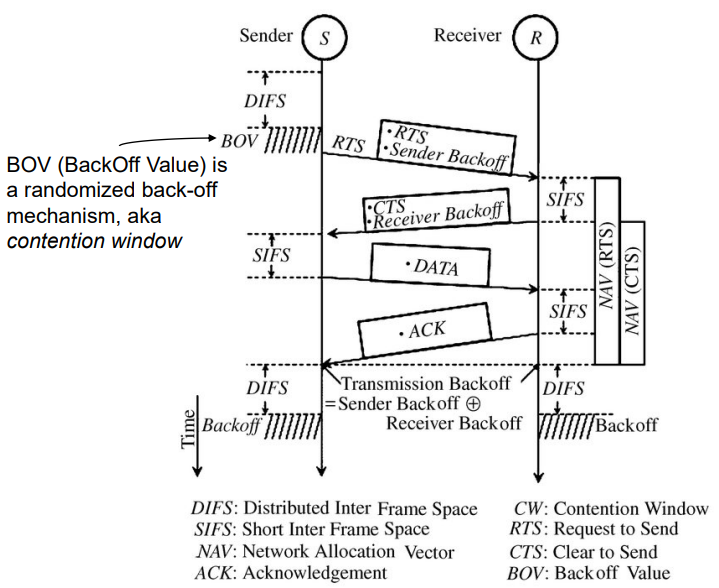
\includegraphics[scale = 0.35]{images/data-sending-procedure.png} 
    \caption{CSMA/CA}
    \label{CSMA/CA}
\end{figure}

\subsubsection{Point Coordinating Function (PCF)/Polling version}
Characteristics:
\begin{itemize}
    \item Access Point has complete control over transmissions
    \item it asks to each node if it has something to transmit $\rightarrow$ managed by round-robin
    $\Rightarrow$ no collisions, ok with many nodes
    \item how it works:
    \begin{enumerate}
        \item AP announces if it supports PCF in the beacon
        \item The AP periodically broadcasts beacons
        \item Nodes use these beacons to learn about AP
        \item The node and the AP authenticate each other:
        \begin{enumerate}
            \item node associates with that AP
            \item node sends an association request management frame\\
            $\rightarrow$ here node announces to the AP if:
            \begin{itemize}
                \item[$\star$] pollable
                \item[$\star$] capable to transmit during the contention free period (CFP)
            \end{itemize}
            \item AP replies with an association response
        \end{enumerate}
    \end{enumerate}
\end{itemize}

\subsubsection{Considerations CSMA}
Some considerations about CSMA:
\begin{itemize}
    \item exposed terminal problem $\rightarrow$ it is not improved
    $\rightarrow$ with CSMA is even worse\\
    $\rightarrow$ enlarge the detection $\Rightarrow$ there are potentially more nodes
    \item it is always better to use RTS/CTS on CSMA/CA and polling versions because:
    \begin{itemize}
        \item[$\rightarrow$] more bandwidth consumed $\rightarrow$ but probability of collision is smaller\\
        $\Rightarrow$ it is an improvement at the cost of limited overhead of transmission
        \item[$\rightarrow$] if data packets are very small (as RTS ones) $\rightarrow$ it is worse
    \end{itemize}
    \item positioning $\rightarrow$ can deal with different MAC layers (802.11, 802.3)
\end{itemize}
\vspace*{0.4cm}
\begin{minipage}{.32 \linewidth}
\begin{tabular}{|c|}
    \hline
    \cellcolor{lightpink}Application\\
    \hline
    \cellcolor{lightred}TCP\\
    \hline
    \cellcolor{lightorange}IP\\
    \hline
    \cellcolor{lightyellow} LLC\\
    \hline
    \cellcolor{lightblue} 802.11 MAC\\
    \hline
    \cellcolor{lightblue} 802.11 PHY\\
    \hline
\end{tabular}
\end{minipage}
\begin{minipage}{.48 \linewidth}
\begin{tabular}{|c|c|}
    \multicolumn{2}{c}{}\\
    \multicolumn{2}{c}{}\\
    \multicolumn{2}{c}{}\\
    \hline
    \multicolumn{2}{|c|}{\cellcolor{lightyellow} LLC}\\
    \hline
    \cellcolor{lightblue} 802.11 MAC & \cellcolor{lightgreen} 802.3 MAC\\
    \hline
    \cellcolor{lightblue} 802.11 PHY & \cellcolor{lightgreen} 802.3 MAC\\
    \hline
\end{tabular}
\end{minipage}
\begin{minipage}{\linewidth}
    \begin{tabular}{|c|}
        \hline
        \cellcolor{lightpink}Application\\
        \hline
        \cellcolor{lightred}TCP\\
        \hline
        \cellcolor{lightorange}IP\\
        \hline
        \cellcolor{lightyellow} LLC\\
        \hline
        \cellcolor{lightgreen} 802.3 MAC\\
        \hline
        \cellcolor{lightgreen} 802.3 PHY\\
        \hline
\end{tabular}
\end{minipage}
\vspace*{0.4cm}
\subsubsection{Synchronization in 802.11}
Characteristics:
\begin{itemize}
    \item AP send beacons in infrastructure networks
    \item beacons are scheduled in beacon interval
    $\rightarrow$ transmission may be delayed\\by CSMA deferral
    \item timestamp contains timer value at transmit time
    \item Power Management approach:
    \begin{itemize}
        \item[$\rightarrow$] allow idle stations to go to sleep $\rightarrow$ save mode stored in AP
        \item[$\rightarrow$] AP buffers packets for sleeping stations
        $\rightarrow$ AP announces which station has packets buffered
        $\rightarrow$ message is sent with TIM\footTIM interval
        \item[$\rightarrow$] power saving station wake up periodically to listen to beacons
        \item[$\rightarrow$] TSF\footTSF assures AP and power saving stations are synchronized
        \item[$\rightarrow$] there is also dTIM $\rightarrow$ less frequently $\rightarrow$  stations give priority to dTIM\\$\rightarrow$ used for broadcasting/multicasting
    \end{itemize}
    \item Scanning:
    \begin{itemize}
        \item[$\rightarrow$] used for
        \begin{itemize}
            \item finding/joining networks
            \item finding a new AP while roaming
            \item initialising a new ad hoc network
        \end{itemize}
        \item[$\rightarrow$] MAC layer uses common mechanism for all physical
        \item[$\rightarrow$] it could be:
        \begin{itemize}
            \item active $\rightarrow$ it looks explicitly for AP\\
            On each channel $\Rightarrow$\\send a probe $\rightarrow$ wait for probe response\\
            send an association request $\rightarrow$ wait for association request response
            \item passive $\rightarrow$ only listen for beacons
        \end{itemize}
    \end{itemize}
\end{itemize}

\subsubsection{Congestion Avoidance (DCF)}
Characteristics:
\begin{itemize}
    \item how it works actually:
    \begin{itemize}
        \item[$\rightarrow$] after DIFS $\rightarrow$ randomly choose a backoff time interval
        \item[$\rightarrow$] Countdown the backoff interval when medium is free\\$\rightarrow$ it goes stand-by if medium becomes busy
        in the range [0,CW]
        \item[$\rightarrow$] When backoff time interval reaches 0 $\rightarrow$ transmit packet (or RTS)
    \end{itemize}
    \item Congestion control $\rightarrow$ dynamically adjusting the CW
    \item Counting down backoff time intervals contributes to MAC overhead
    \item Binary Exponential Backoff $\rightarrow$ a node fails to receive CTS\\
    $\Rightarrow$ it double up the CW (typically max size is 1024)\\
    $\rightarrow$ when node successfully completes transfer $\Rightarrow$ it restores CW to $\text{CW}_\text{min}$
    \item So about the dimension of CW:
    \begin{itemize}
        \item[$\rightarrow$] Large CW $\Rightarrow$ large backoff time intervals $\Rightarrow$
        can result in larger overhead
        \item[$\rightarrow$] Small CW $\Rightarrow$ probabilistically to a larger number of collisions
    \end{itemize}
\end{itemize}
\subsubsection{MILD Algorithm MACAW}
Characteristics:
\begin{itemize}
    \item node fails to receive CTS $\rightarrow$ it multiplies CW by 1.5\\
    $\Rightarrow$ less aggressive than 802.11 which multiplies by 2
    \item node successfully completes a transfer $\rightarrow$
    it reduces CW by 1\\ $\Rightarrow$ more conservative than 802.11
    where CW is restored to $\text{CW}_\text{min}$
    \item 802.11 reduces cw much faster than it increases it
    \item MACAW: cw reduction slower than the increase\\
    $\Rightarrow$ Exponential Increase and Linear Decrease
    \item  MACAW can avoid wild oscillations of CW when congestion is high
\end{itemize}

\subsubsection{Fairness Issue}
Characteristics:
\begin{itemize}
    \item Definition:
    \begin{itemize}
        \item[$\rightarrow$] nodes should receive equal bandwidth
        \item[$\rightarrow$] bandwidth should be tailored to how much they want to transmit\\
        $\Rightarrow$ otherwise waste of time/bandwidth
    \end{itemize}
    \item unfairness $\rightarrow$ one node has backed
    off much more than some other node\\($\approx$ channel dominance)\\
    $\rightarrow$ A transmits many packets before B is transmitting its first
    \item how MACAW tries to solve:
    \begin{enumerate}
        \item a node transmits a packet $\rightarrow$ it appends on packet its current
        CW value
        \item All nodes hear CW value $\rightarrow$ use it for their future
        transmission attempts
        \item The effect is to reset all competing nodes to the same level
    \end{enumerate}
    \item Weighted Fair Queueing $\rightarrow$ it is assigned a weight to each node\\
    $\Rightarrow$ bandwidth used by each node $\rightarrow$ proportional to the weight
    assigned
    \newpage
    \item Distributed Fair Scheduling (DFS)
    \begin{itemize}
        \item[$\rightarrow$] it is fully distributed algorithm for achieving weighted
        fair queueing
        \item[$\rightarrow$] it works well on a LAN
        \item[$\rightarrow$] how it works:
        \begin{enumerate}
            \item Chooses backoff intervals proportional to
            packet size/weight
            \item DFS attempts to follow the centralized Self-Clocked
            Fair Queueing
        \end{enumerate}
    \end{itemize}
\end{itemize}
\vspace*{0.4cm}
\begin{figure}[!h] 
    \centering 
    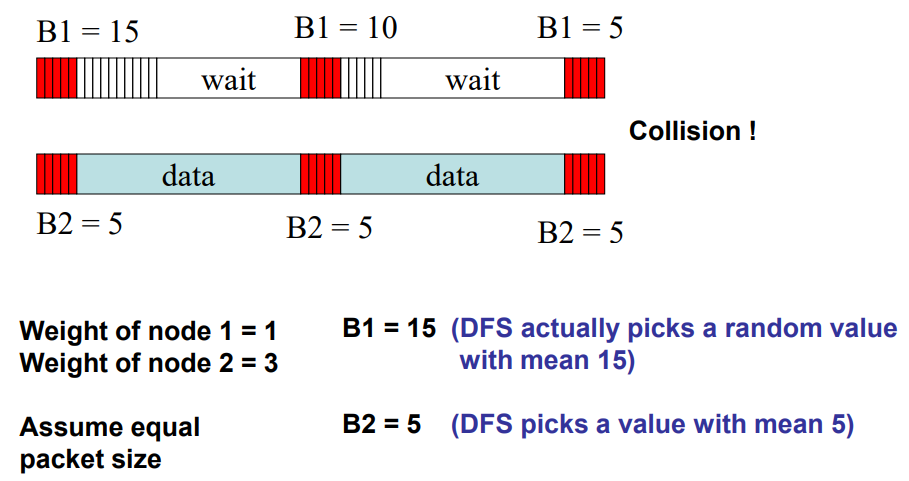
\includegraphics[scale = 0.35]{images/DFS.png} 
    \caption{Distributed Fair Scheduling (DFS)}
    \label{DFS}
\end{figure}